\documentclass[11pt,a4paper]{article}
\usepackage[margin=0.8in]{geometry}
\usepackage{tikz}
\usepackage{pgf-umlcd}
\usepackage{fontspec}
\usepackage{xcolor}
\usepackage{amsfonts}
\usepackage{amsmath}
\usepackage{listings}

% Configure emoji font for XeLaTeX (vector-based for better compatibility)
\newfontfamily\emojifont{Segoe UI Emoji}[
    Scale=1.0
]

% Create convenient emoji command
\newcommand{\emoji}[1]{{\emojifont #1}}

\usetikzlibrary{shapes,arrows,positioning,fit,backgrounds,decorations.pathmorphing,calc,shadows,matrix,chains}

\title{PeiDocker Terminal GUI - Simple Mode Wizard Design Test}
\author{Claude Code}
\date{\today}

\definecolor{primaryblue}{RGB}{51,122,183}
\definecolor{successgreen}{RGB}{92,184,92}
\definecolor{warningorange}{RGB}{240,173,78}
\definecolor{dangered}{RGB}{217,83,79}
\definecolor{lightgray}{RGB}{248,248,248}
\definecolor{darkgray}{RGB}{85,85,85}
\definecolor{infoblue}{RGB}{91,192,222}

\tikzset{
    % Screen frame style
    screen/.style={
        rectangle, draw=primaryblue, thick, fill=lightgray!30,
        minimum width=14cm, minimum height=10cm,
        rounded corners=5pt
    },
    % Input field style
    inputfield/.style={
        rectangle, draw=darkgray, fill=white,
        minimum width=6cm, minimum height=0.8cm,
        rounded corners=2pt
    },
    % Button styles
    primarybtn/.style={
        rectangle, draw=primaryblue, thick, fill=primaryblue!30,
        minimum width=2cm, minimum height=0.8cm,
        rounded corners=3pt, font=\bfseries
    },
    secondarybtn/.style={
        rectangle, draw=darkgray, fill=lightgray,
        minimum width=2cm, minimum height=0.8cm,
        rounded corners=3pt
    },
    % Warning style
    warning/.style={
        rectangle, draw=warningorange, fill=warningorange!20,
        text width=12cm, rounded corners=3pt,
        font=\footnotesize
    }
}

\begin{document}

\maketitle

\section{Simple Mode Test}

This is a test document to verify XeLaTeX compilation with emoji support.

\subsection{Basic Emoji Test}

Here are some basic emojis using the emoji command:
\begin{itemize}
    \item Warning: \emoji{⚠}
    \item Checkmark: \emoji{✓}
    \item Cross: \emoji{✗}
\end{itemize}

\subsection{Simple Screen Example}

\begin{figure}[htbp]
\centering
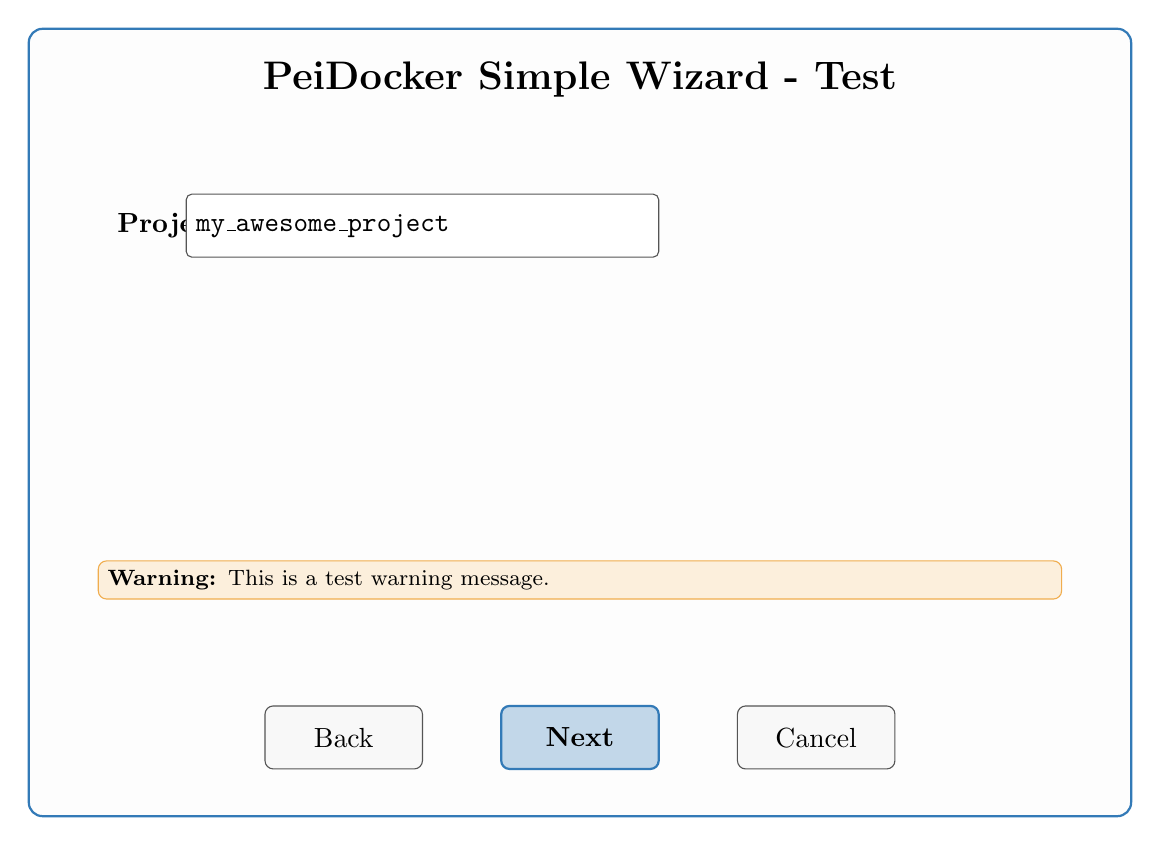
\begin{tikzpicture}

% Main screen frame
\node[screen] (frame) at (0,0) {};
\node[anchor=north] at (0,4.7) {\Large\textbf{PeiDocker Simple Wizard - Test}};

% Project name input
\node[anchor=west, font=\bfseries] at (-6,2.5) {Project Name:};
\node[inputfield] (projname) at (-2,2.5) {};
\node[anchor=west, font=\ttfamily] at (-5,2.5) {my\_awesome\_project};

% Warning area (conditional)
\node[warning] at (0,-2) {
    \textbf{Warning:} This is a test warning message.
};

% Navigation buttons
\node[secondarybtn] at (-3,-4) {Back};
\node[primarybtn] at (0,-4) {Next};
\node[secondarybtn] at (3,-4) {Cancel};

\end{tikzpicture}
\caption{Test Screen Layout}
\end{figure}

\section{Emoji Font Test}

Direct emoji usage:
\begin{itemize}
    \item \emoji{😊} Happy face
    \item \emoji{🚀} Rocket
    \item \emoji{⚠} Warning sign
    \item \emoji{✓} Check mark
\end{itemize}

\end{document}